\chapter{Theoretical foundation and literature review}
\label{cap:cap2}

% (aproximativ 5 pagini)
%\footnote{\textit{Template}-ul inițial a fost construit similar celui dezvoltat de George VIERIU, disponibil la \url{https://ac.tuiasi.ro/studenti/didactic/finalizare-studii/finalizare-studii-calculatoare/finalizare-studii-calculatoare-ghidul-studentului/}}

% \begin{itemize}
%     \item Prezentarea conceptelor și teoriilor relevante pentru tema abordată.
%     \item Prezentarea succintă și comparativă privind realizările actuale pe aceeași temă din literatura de specialitate.
%     \item Analiza tipurilor de soluții/aplicații existente din respectiva categorie a temei.
%     \item Identificarea lacunelor în stadiul actual și cele referitoare la soluțiile existente.
%     \item Elaborarea specificațiilor privind caracteristicile așteptate de la aplicație.
% \end{itemize}

% Lucrările utilizate în dezvoltarea proiectului de diplomă și în redactarea tezei vor fi citate corespunzător în cadrul prezentului document. Această citare trebuie să fie o interpretare sau o descriere proprie autorului prezentei teze asupra ideii/soluției/conceptului prezentat în lucrarea sursă și \textbf{\textit{nu}} o preluare mot-a-mot sau o traducere directă. O posibilă excepție de la această regulă se poate face în cazul rezultatelor teoretice importante, cum ar fi, de exemplu, definițiile, teoremele sau algoritmii suport. În textul asociat citării este recomandat să includeți, de asemenea, și o frază prin care să realizați legătura cu lucrarea proprie. Teza capătă în acest fel consistență și evitați ideea de citare bulk, „doar ca să fie". În continuare vă prezentăm un scurt exemplu.

% \todo[inline]{TO DO: Aici ar trebui să introduc o referință bibliografică deoarece ceea ce am scris nu este ideea mea}

% Pornind de la modelul REST propus de Fielding în \cite{thesis:fielding:2000} și considerând specificațiile protocolului HTTP \cite{misc:web:rfc7231}, Archip et. al. demonstrează în \cite{inproc:archip:restful:2018} faptul că o utilizare greșită a modelului amintit poate conduce la o slăbire a securității unui server. Un alt aspect important care trebuie considerat cu privire la securitatea sistemelor informatice este legat de utilizatori. Acest subiect este tratat pe larg în \cite{incollection:ARASEC2020}.

% Mironeanu et. al. propun o nouă abordare pentru monitorizarea și prevenția atacurilor cibernetice \cite{art:mironeanu:ECAD:2021}. Soluția utilizează tehnici de tip AI/ML și pe un sistem de votare ponderat cu scopul de determina dacă un acces în rețea este un acces normal sau un eventual atac. Pornind de la noțiunile descrise în \cite{art:mironeanu:ECAD:2021}, lucrarea de față își propune îmbunătățirea detecției atacurilor de tip \textit{flood}.

% Un exemplu de intrare bibliografică pentru un \textit{tech report} este în \cite[p.~13]{IEEEexample:techreptypeii} (numărul paginii este trecut explicit în sursă). Bineînțeles, nu putem discuta despre configurările și instalările unor sisteme Cloud Computing \cite[p.~113]{book:marinescu:2018}, dacă nu considerăm și sistemele de operare suport sau gazdă \cite{book:operating_systems:2014}. În cazul în care dorim să referim o pagină web care nu se încadrează în categoriile carte, articol, raport tehnic, putem să utilizăm o intrare de tip \verb|misc| în bibliografie. Recomandarea este să utilizăm documente Web publicate de companii importante (precum IBM, RedHat, Apple, etc.) sau personalități recunoscute, precum Bruce Schneier \cite{misc:web:schneier2021}.

% (Figura \ref{fig:puterea_furnizata_pe_cm_cub})

% \begin{figure}[H]
%     \centering
%     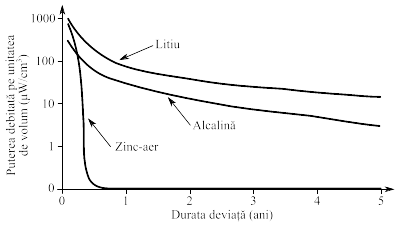
\includegraphics[width=0.6\textwidth]{continut/capitol2/figuri/puterea_furnizata_pe_cm_cub.png}
%     \caption{Puterea furnizată pe cm\textsuperscript{3} relativă la durata de viață pentru trei tipuri de baterii.}
%     \label{fig:puterea_furnizata_pe_cm_cub}
% \end{figure}


% \section{Exemplu de subcapitol nivel 1}
% \label{cap:cap2:ex-subcapitol}

% (Figura \ref{fig:r2_d2})

% \begin{figure}[t]
%     \centering
%     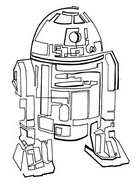
\includegraphics[width=0.25\textwidth]{continut/capitol2/figuri/r2_d2.png}
%     \caption{R2-D2\protect\footnotemark}
%     \label{fig:r2_d2}
% \end{figure}
% \footnotetext{imagine preluată de pe un site web care nu „merită” trecut la bibliografie \url{https://www.shutterstock.com/}}

% \subsection{Exemplu de subcapitol nivel 2}
% \label{cap:cap2:ex-supcapitol:nivel2}

% (Figura \ref{fig:yoda})

% \begin{figure}[H]
%     \centering
%     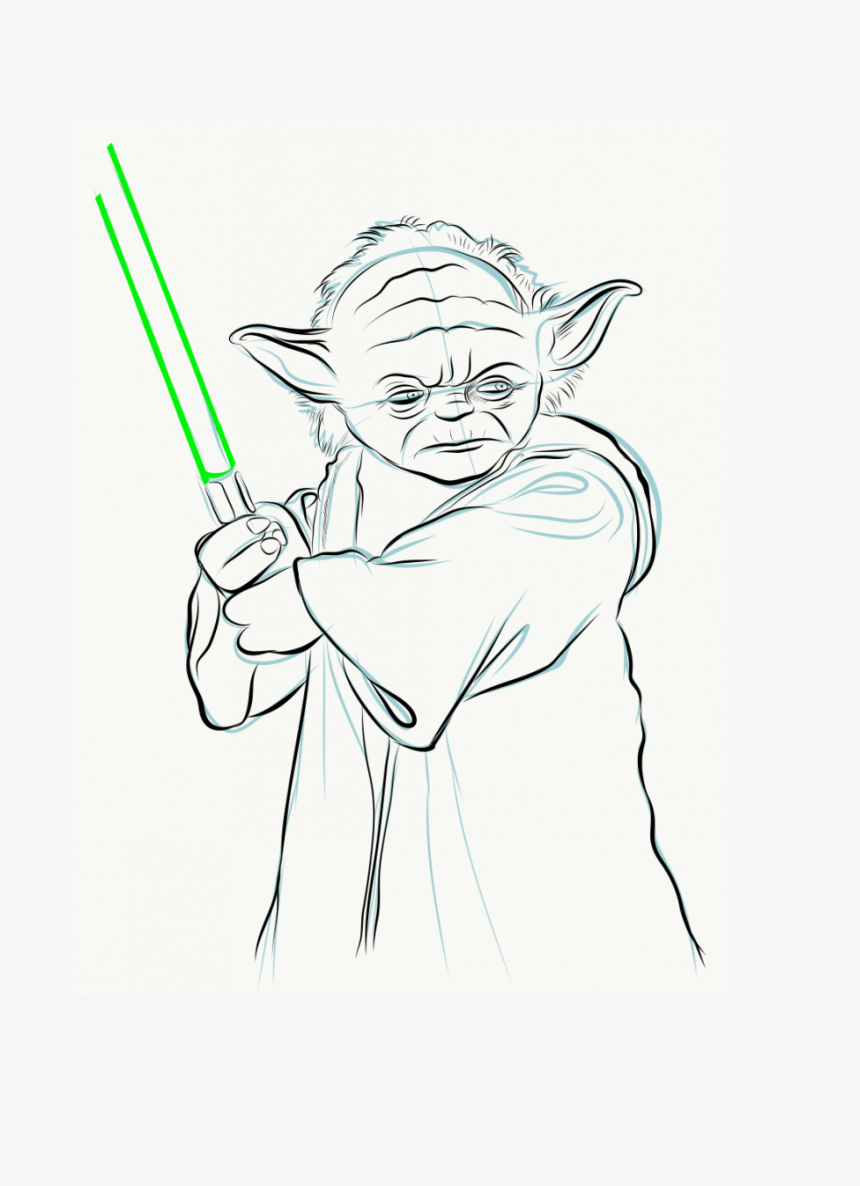
\includegraphics[width=0.3\textwidth]{continut/capitol2/figuri/yoda.png}
%     \caption{Yoda\protect\footnotemark}
%     \label{fig:yoda}
% \end{figure}
% \footnotetext{imagine preluată de pe un site web care nu „merită” trecut la bibliografie \url{https://www.pngitem.com/}}


% \subsubsection{Exemplu de subcapitol nivel 3}
% \label{cap:cap2:ex-subcapitol:nivel2:nivel3}

% Următoarele e fără label FTW, decât să demonstrez gen!\footnote{Dacă vă prindem cu astfel de exprimări, vă scădem 2 puncte!!!}

% \section{Nivel 1}
% \label{cap:cap2:nivel1}

% \subsection{Nivel 2}
% \label{cap:cap2:nivel1:nivel2}

% Ghilimelele se pun înainte și după reproducerea unui text. Se pun între semnele citării cuvintele sau grupurile de cuvinte citate ironic sau care redau atitudinea rezervată ori dezaprobatoare a autorului față de realitățile pe care le desemnează respectivele cuvinte. Se obișnuiește să se pună între ghilimele titlurile operelor literare de artă sau științifice, ale publicațiilor, numele instituțiilor, firmelor etc. atunci când aceste titluri sunt reproduse într-o frază. 
% Atenție: Ghilimelele limbii engleze (“ ”) sunt diferite de ghilimelele limbii române („ ”)!
% Observație: Documentele tehnice au adoptat din sintaxa limbajelor de programare ghilimelele duble (") pentru a evidenția șirurile de caractere în text și ghilimelele simple (') pentru evidențierea caracterelor. De exemplu: "acesta este un șir de caractere", acesta este caracterul 'x'.

% \subsubsection{Nivel 3}
% \label{cap:cap2:nivel1:nivel2:nivel3}

% Oricum, mai departe de \verb|#.#.#.#| \textbf{\textit{NU}} trebuie să se ajungă :P.

This chapter reviews the theoretical concepts and current research relevant to biomass estimation from image and remote-sensing data. It begins with the role of biomass estimation in precision agriculture and the evolution from traditional destructive sampling to image-based methods. It then discusses classical machine learning approaches, deep learning methods, and recent work on transfer learning, domain adaptation, and synthetic data. Special attention is given to validation practices, because the reliability of reported performance is central to the present thesis. Finally, the chapter identifies gaps in the current literature and formulates the expected characteristics of an evaluation-oriented solution.

\section{Biomass Estimation and the Role of Remote Sensing}

Biomass estimation is a key task in precision agriculture. It supports the monitoring of crop and pasture status, the assessment of productivity, and the optimization of resource management. In grazing systems, for example, above-ground biomass is used to estimate forage availability and to plan livestock rotation. In cropping systems, biomass measurements can indicate plant health, stress, and yield potential.

Traditionally, biomass is measured by destructive sampling: vegetation is cut, dried, and weighed. Although accurate at the plot level, this method is labor-intensive, time-consuming, and cannot be applied continuously over large areas. Remote sensing has therefore become an attractive alternative. Satellite imagery offers wide spatial coverage, while unmanned aerial vehicles provide very high spatial resolution and flexible acquisition timing. Ground-based cameras, including smartphones, are also used because they are inexpensive and easy to deploy.

The available sensor types differ in their information content. RGB imagery captures visible color and texture, while multispectral and hyperspectral sensors record reflectance in additional spectral bands that are often related to vegetation properties. However, the choice of sensor also affects cost, processing complexity, and transferability. These trade-offs are important for real-world agricultural applications.

The present thesis focuses on RGB imagery because it is accessible and practical. At the same time, it recognizes that RGB-based models may face challenges when visual conditions change across time and space. This motivates the investigation of validation strategies that can estimate how well a model will perform under such changes.

\section{Classical Machine Learning Approaches}

A large body of research has applied classical machine learning to biomass estimation. These approaches typically combine manually designed features with models such as linear regression, random forests, support vector regression, or gradient boosting. The features are usually derived from spectral bands, vegetation indices, texture descriptors, and sometimes environmental variables such as soil properties or weather data.

Several studies illustrate the diversity of this line of work. Sharma et al.~\cite{sharma2022oats} estimated above-ground biomass in oats using remote-sensing features and machine learning. Wang et al.~\cite{wang2022grassland} analyzed grassland biomass with machine learning models and multisource data. Vahidi et al.~\cite{vahidi2023sentinel} used Sentinel imagery to estimate biomass in pasture and bale grazing systems. Hyperspectral data were employed for biomass monitoring by Huang et al.~\cite{huang2022hyperspectral} and Oliveira et al.~\cite{oliveira2023hyperspectral}, who showed that narrow spectral bands can contain important information about vegetation status.

Other studies have focused on feature importance and model automation. Zhao et al.~\cite{zhao2024feature} investigated feature-importance analysis for predicting grassland biomass and nutrient-related parameters. Li et al.~\cite{li2022automl} applied automated machine learning to biomass and crop-yield prediction, reducing the need for manual model selection. Further applications include alpine grassland mapping~\cite{shi2023alpine}, dry matter estimation in cattle grazing systems~\cite{defalque2024drymatter}, belowground biomass prediction from aboveground biomass and soil properties~\cite{zhao2025belowground}, and cover crop prediction~\cite{poudel2025cover}.

These studies demonstrate that classical machine learning can produce accurate predictions when the features are well chosen and the sensor characteristics are stable. However, the main limitation is their dependence on expert feature engineering. The selected features may not transfer well to new locations, sensors, or acquisition dates. This limitation is directly relevant to the present thesis: if the relationship between features and biomass changes across time, a model that performs well under random validation may fail in a new campaign. The Ridge baseline used in this work belongs to this classical family but operates on visual embeddings rather than handcrafted features, allowing a direct comparison with a more flexible neural model.

\section{Deep Learning Approaches}

Deep learning methods have become increasingly popular for biomass estimation because they can learn spatial, spectral, and semantic representations directly from image data. Convolutional neural networks are the most common architecture, but recent work also uses vision transformers and segmentation models.

Several studies have used convolutional networks for biomass-related tasks. Vawda et al.~\cite{vawda2024cnn} estimated dry-season grass biomass from Sentinel-2 data. Castro et al.~\cite{castro2020deep} developed a deep learning approach for forage biomass phenotyping from UAV RGB imagery. Zheng et al.~\cite{zheng2022strawberry} combined canopy delineation with biomass prediction in strawberry fields. Vahidi et al.~\cite{vahidi2023rgbuav} estimated pasture biomass from ultra-high-resolution UAV imagery. Other applications include grass weed detection and yield-related analysis~\cite{liu2024weed}, pasture biomass estimation from digital photographs~\cite{woodrow2023continuous}, segmentation-based forage analysis~\cite{moreno2025segmentation}, temporal modeling with vegetation indices~\cite{wagle2024timeseries}, and uncertainty-aware edge deployment~\cite{zawish2024edge}. Karila et al.~\cite{karila2022grass} demonstrated that deep neural architectures combined with drone remote sensing can estimate grass quality and quantity parameters.

A notable recent contribution is the CSIRO Image2Biomass dataset introduced by Liao et al.~\cite{liao2025estimating}. This public benchmark contains top-view pasture images with multiple biomass components and has been used in a Kaggle competition. It serves as the foundation for the present study because it provides a realistic setting with a hidden test set from different years.

Deep learning reduces the need for manual feature design and often improves accuracy on complex visual tasks. However, these models are data-hungry and can easily overfit when the training set is small or homogeneous.

DINOv3~\cite{simeoni2025dinov3} is a self-supervised vision transformer trained with a self-distillation objective. Unlike supervised ImageNet-pretrained backbones, DINOv3 learns visual representations without requiring manual labels. These representations have been shown to transfer well to downstream tasks, including fine-grained image classification and regression.

In this work, DINOv3 is used as a frozen feature extractor. This means that the backbone weights are kept fixed and only a lightweight regression head is optimized. This choice is methodologically important: it isolates the effect of the validation protocol from the effect of representation learning. If the backbone were fine-tuned, the model could adapt to the public data distribution and introduce an additional source of variation that would be difficult to separate from the validation effect.

\section{Transfer Learning, Domain Adaptation, and Synthetic Data}

A growing branch of research addresses the problem of distribution shift by using transfer learning, domain adaptation, or synthetic data. These methods explicitly recognize that models trained on one region or period may not perform well on another.

Wang et al.~\cite{wang2023transfer} proposed a transfer learning framework for sorghum biomass prediction using UAV data and genetic markers. Their approach shows that information from related tasks or modalities can improve generalization. Albert et al.~\cite{albert2022domain} investigated unsupervised domain adaptation for herbage biomass estimation from drone imagery, aiming to reduce the gap between source and target domains. Sapkota et al.~\cite{sapkota2022synthetic} explored synthetic images for weed detection and biomass estimation in cotton, which is especially useful when labeled data are scarce.

These adaptation strategies implicitly acknowledge that distribution shift exists and that standard training may not be sufficient. However, the evaluation of such methods is often performed using random splits or a single held-out set. This can lead to optimistic conclusions because the adaptation itself may overfit the specific validation setting. The present thesis differs from these works by focusing not on a new adaptation technique, but on how validation protocols themselves influence performance estimation. In other words, before improving the model, we ask whether the evaluation procedure already provides a misleading picture of real-world performance.

\section{Validation and Generalization under Spatiotemporal Dependence}

A central assumption of standard cross-validation is that the data points are independent and identically distributed. Under this assumption, randomly splitting the dataset into training and validation folds gives an unbiased estimate of the model's performance on unseen data from the same distribution.

\subsection{Distribution Shift in Agricultural Image Data}

In the standard supervised learning setting, the training and test data are assumed to be drawn independently from the same distribution. Under this assumption, random cross-validation provides an approximately unbiased estimate of test performance.

In agricultural and remote sensing applications, this assumption is frequently violated. Images collected on the same day share illumination, weather, vegetation stage, and sensor state. Images collected at nearby locations share soil properties and vegetation communities. These shared factors create spatial and temporal autocorrelation. If correlated observations appear in both training and validation folds, the model can exploit nuisance dependencies instead of learning the true image-to-biomass relationship, producing an artificially high validation score.

Three forms of distribution shift are particularly relevant. Covariate shift occurs when the input distribution changes between training and deployment, for example because the visual appearance of pasture changes with season. Label shift occurs when the distribution of biomass values changes, for example between a dry and a wet year. Concept shift occurs when the relationship between images and biomass changes, for example because of different mixtures of species or management practices. In the Image2Biomass benchmark, the hidden test set contains images from different years and locations, so all three forms of shift are plausible.

\subsection{Grouped Cross-Validation and Data Leakage}

Random cross-validation assumes that observations can be exchanged freely between training and validation folds. Grouped cross-validation relaxes this assumption by defining groups of observations that must not be split across folds. A group is typically a date, a location, a field, or a combination of date and location.

The motivation is to reduce data leakage. When two images are acquired on the same date at the same site, they share environmental and acquisition conditions. If one image is used for training and the other for validation, the model can rely on these shared conditions instead of generalizing to genuinely new conditions. Grouping by date prevents this specific form of temporal leakage. Grouping by date and state further reduces spatial leakage, but at the cost of smaller effective training sets and higher variance.

Leave-one-out variants, such as Leave-One-Date-Out or Leave-One-Period-Out, represent the strictest form of grouped evaluation. They train on all data except one group and test on the held-out group. Although they provide a strong test of generalization, they are computationally expensive and may be unstable when groups are small.

\subsection{Empirical Evidence and Relevance}

Roberts et al.~\cite{roberts2017cross} documented the bias of random cross-validation under spatial autocorrelation in ecological modeling. Ploton et al.~\cite{ploton2020spatial} similarly showed that random validation can overestimate model performance in remote sensing applications when spatial structure is present. Their analyses demonstrate that grouped or blocked validation is necessary to obtain more realistic estimates.

These findings are highly relevant to the present work. The CSIRO Image2Biomass public split is organized in collection campaigns, and the hidden test set comes from different years and locations. As a result, random cross-validation is expected to overestimate the hidden-test performance. The present thesis extends the work of Roberts et al.~\cite{roberts2017cross} and Ploton et al.~\cite{ploton2020spatial} by quantifying protocol-specific optimism relative to an independent hidden test set. It also analyzes how different validation protocols affect model-selection decisions, such as the stopping epoch.

\section{The CSIRO Image2Biomass Benchmark and Its Evaluation Challenge}

The CSIRO Image2Biomass dataset~\cite{liao2025estimating} provides a concrete case study for the validation problem. The public split contains images from 2015 collected in multiple Australian states. The hidden test set contains images from 2014 and 2016 and does not include metadata. The official metric is the weighted coefficient of determination $R^2_w$, which combines five biomass components with different weights.

This design creates a realistic but challenging evaluation scenario. The public data are small and temporally clustered, while the hidden data cover different years. As a result, any validation protocol based only on the public data may underestimate the difficulty of the hidden test. The present study uses this benchmark to compare three validation strategies: Random CV, Date CV, and Date-State CV. The key quantity of interest is the optimism gap, defined as the difference between local validation performance and hidden-test performance.

A state-only cross-validation protocol was not included. The public dataset contains images from only four Australian states, with a highly unbalanced distribution: Tasmania contributes 138 images, Victoria 112, New South Wales 75, and Western Australia 32. This imbalance makes a five-fold state-based split impractical, because some folds would contain very few images and the effective training set size would vary strongly across folds. Moreover, Date-State CV already introduces spatial constraints, since grouping by date and state prevents images from the same acquisition campaign and the same geographic region from being split across training and validation. Therefore, Date-State CV was preferred as the spatiotemporal protocol.

\section{Identified Gaps and Expected Characteristics of an Evaluation-Oriented Solution}

\begin{table}[htbp]
\centering
\caption{Summary of related work on biomass estimation and validation under spatiotemporal structure.}
\label{tab:related_work}
\small
\renewcommand{\arraystretch}{1.5}
\begin{threeparttable}
\begin{tabular}{p{2.0cm}p{2.5cm}p{2.8cm}p{2.6cm}p{1.8cm}p{2.5cm}}
\hline
\textbf{Study} & \textbf{Task / data} & \textbf{Approach} & \textbf{Validation protocol} & \textbf{Independent hidden test?} & \textbf{Main limitation} \\
\hline
Sharma et al.~\cite{sharma2022oats} & Above-ground biomass in oats & Classical ML on remote-sensing features & Random CV & No & No grouped validation \\
Castro et al.~\cite{castro2020deep} & Forage biomass from UAV RGB & CNN & Random split & No & Likely spatial leakage \\
Liao et al.~\cite{liao2025estimating} & Pasture biomass, Image2Biomass & Dataset introduction and benchmark & Hidden test provided by competition & Yes (benchmark set) & No analysis of validation protocols on the public split \\
Roberts et al.~\cite{roberts2017cross} & Ecological modeling & Random forest & Random vs spatial CV & No & Demonstrated overestimation, no hidden test \\
Ploton et al.~\cite{ploton2020spatial} & Remote sensing biomass & Machine learning & Spatial CV & No & No independent hidden test \\
This work & Pasture biomass, Image2Biomass & Ridge + MLP on frozen DINOv3 & Random, Date, Date-State CV + hidden test & Yes (Kaggle submission) & Quantifies optimism gap under protocol changes \\
\hline
\end{tabular}
\begin{tablenotes}
\small
\item ``Independent hidden test'' means that the test labels are not available during model development and are used only once for final evaluation. A separate test set from a different period or location may be independent in distribution, but if its labels are accessible during hyperparameter tuning, model selection, or early stopping, it does not constitute a hidden evaluation set. The CSIRO Image2Biomass benchmark is particularly valuable in this regard because it evaluates submissions on a hidden test set through the Kaggle platform, preventing direct access to the test labels during model development.
\end{tablenotes}
\end{threeparttable}
\end{table}

Table~\ref{tab:related_work} summarizes the studies most relevant to the relationship between biomass estimation and validation methodology. The comparison highlights that few studies combine structured validation protocols with evaluation on a hidden-label benchmark. The Image2Biomass competition is particularly valuable in this regard because its hidden test set enables a direct assessment of the discrepancy between local validation performance and unseen-data performance.

From the reviewed literature, several gaps emerge.

\begin{itemize}
    \item Most biomass estimation studies focus on improving predictive accuracy, while the reliability of the validation procedure receives little attention.
    \item Random cross-validation remains the default evaluation strategy, even when the data contain strong temporal or spatial structure.
    \item Few studies compare multiple validation protocols under identical experimental conditions.
    \item Few studies evaluate biomass-estimation models using a hidden-label test set that allows the direct quantification of validation optimism.
    \item The relationship between per-target biomass components and validation protocol sensitivity is rarely analyzed.
    \item The effect of validation on model-selection decisions, such as early stopping, is often ignored.
\end{itemize}

These gaps motivate the characteristics expected from the solution developed in this thesis.

An evaluation-oriented solution should:

\begin{itemize}
    \item use a common experimental pipeline in which only the data-splitting strategy changes;
    \item employ a fixed feature extractor to isolate the effect of the validation protocol from representation learning;
    \item include at least two predictive models with different complexities to test whether validation effects are model-dependent;
    \item implement random, temporal, and spatiotemporal validation protocols;
    \item report local performance together with hidden-test performance and the optimism gap;
    \item analyze per-target behavior in addition to the aggregated metric;
    \item include a stricter temporal evaluation, such as Leave-One-Period-Out, to investigate generalization difficulty within the available data;
    \item provide reproducibility through fixed random seeds and modular implementation.
\end{itemize}

These characteristics are operationalized in Chapter~3, where the proposed solution is described, and evaluated in Chapter~4, where the results are presented. By satisfying these requirements, the thesis does not propose yet another biomass prediction model, but instead contributes a systematic analysis of how evaluation methodology influences the perceived performance of such models.